%%%%%%%%%%%%%%%%%%%%%%%%%%%%%%%%%%%%%%%%%%%%%%%%%%%%%%%%%%%%%%%%%%%
% Background
% Year:
% 2016、2017
% Team:
% Wolverine、RCPL
% Members: 
% Dexter Chen(Wolverine/2016), Eric Chang(Wolverine/2016), Eric Lee(Wolverine/2016), 
% Jacky Wu(Wolverine/2016), Karthick Mani(Wolverine/2016), Kenvin Lo(Wolverine/2016), 
% Yu-cheng Chen(Wolverine/2016), Paul Lin(RCPL/2017)
% (Format:Name(Team/Year))
% Relative files:
% Main.tex, Background_Information_retrieval_on_existing_database.tex, Library.bib, Wolverine_Background_Chart_1.png
% Note: 
% Do not compile this file compile Main.tex to get the pdf file instead.
%%%%%%%%%%%%%%%%%%%%%%%%%%%%%%%%%%%%%%%%%%%%%%%%%%%%%%%%%%%%%%%%%%%
	
\subsection{Information retrieval on existing database}
	We live in the time when technology develops rapidly. Information grows in an exponential rate. 
	Tague1981\cite{Tague1981} forecaster the further into the future we go, the fewer the additional number of first-rate publications. 
	Since the information increases from linear growth to exponential growth, we can't rely on the old ways to find the information we need. 
	Instead, we need new information retrieval methods to handle the big amount of data systematically. 
	
	However, most of the information retrieval methods such as search engine cannot search everything on the web. 
	Grehan2002\cite{Grehan2002} claimed a search engine which can only search the subset of the web it has ‘captured’ and included in its own database. 
	Therefore, we need to create a database to store these data and automatically update them.
	There are several online libraries currently available for us to get the academic articles or periodicals we need.
	Besides, they can be roughly divided into three groups according to the way they store articles based on the division used by National Taiwan University Library.

\paragraph{Index libraries}
	These kind of libraries store the index and abstract of the articles.
	They don't provide the full-text documents directly, but they may provide the links to the publisher websites of articles.
	Besides, they can be categorized by the type of articles they include.
	
	\begin{itemize}		
		\item\textbf{Comprehensive topics}\\Libraries such as Web of Science, Scopus, Google Scholar...
		\item\textbf{Specialized topics}\\Libraries such as Compendex, BIOSIS Previews, PubMed, MEDline...		
	\end{itemize}
	
\paragraph{Publisher libraries}
	These libraries are created by the publishers themselves, so they provide the newest and complete the documents directly.
	Besides, they can also be categorized by the type of articles they include.
	
	\begin{itemize}		
		\item\textbf{Comprehensive topics}\\Libraries such as Science Direct, Springer Link, Wiley Online Library...
		\item\textbf{Specialized topics}\\Libraries such as Nature.com, Emerald Management Xtra, IEEE Xplore...	
	\end{itemize}
	
\paragraph{Aggregator libraries}
	These libraries do not publish the articles by themselves, but sometimes they still provide users with the full-text articles.
	The way they do this is to negotiate with some of the publisher libraries and get the authorization of the articles.
	Libraries such as EBSCOhost, ProQuest, JSTOR...

	The comparison between these libraries can be found on Figure \ref{WBC1}.
	On the next section we will discuss about more details about some of the existing libraries.

\begin{figure*}[htb]
	\begin{center}
		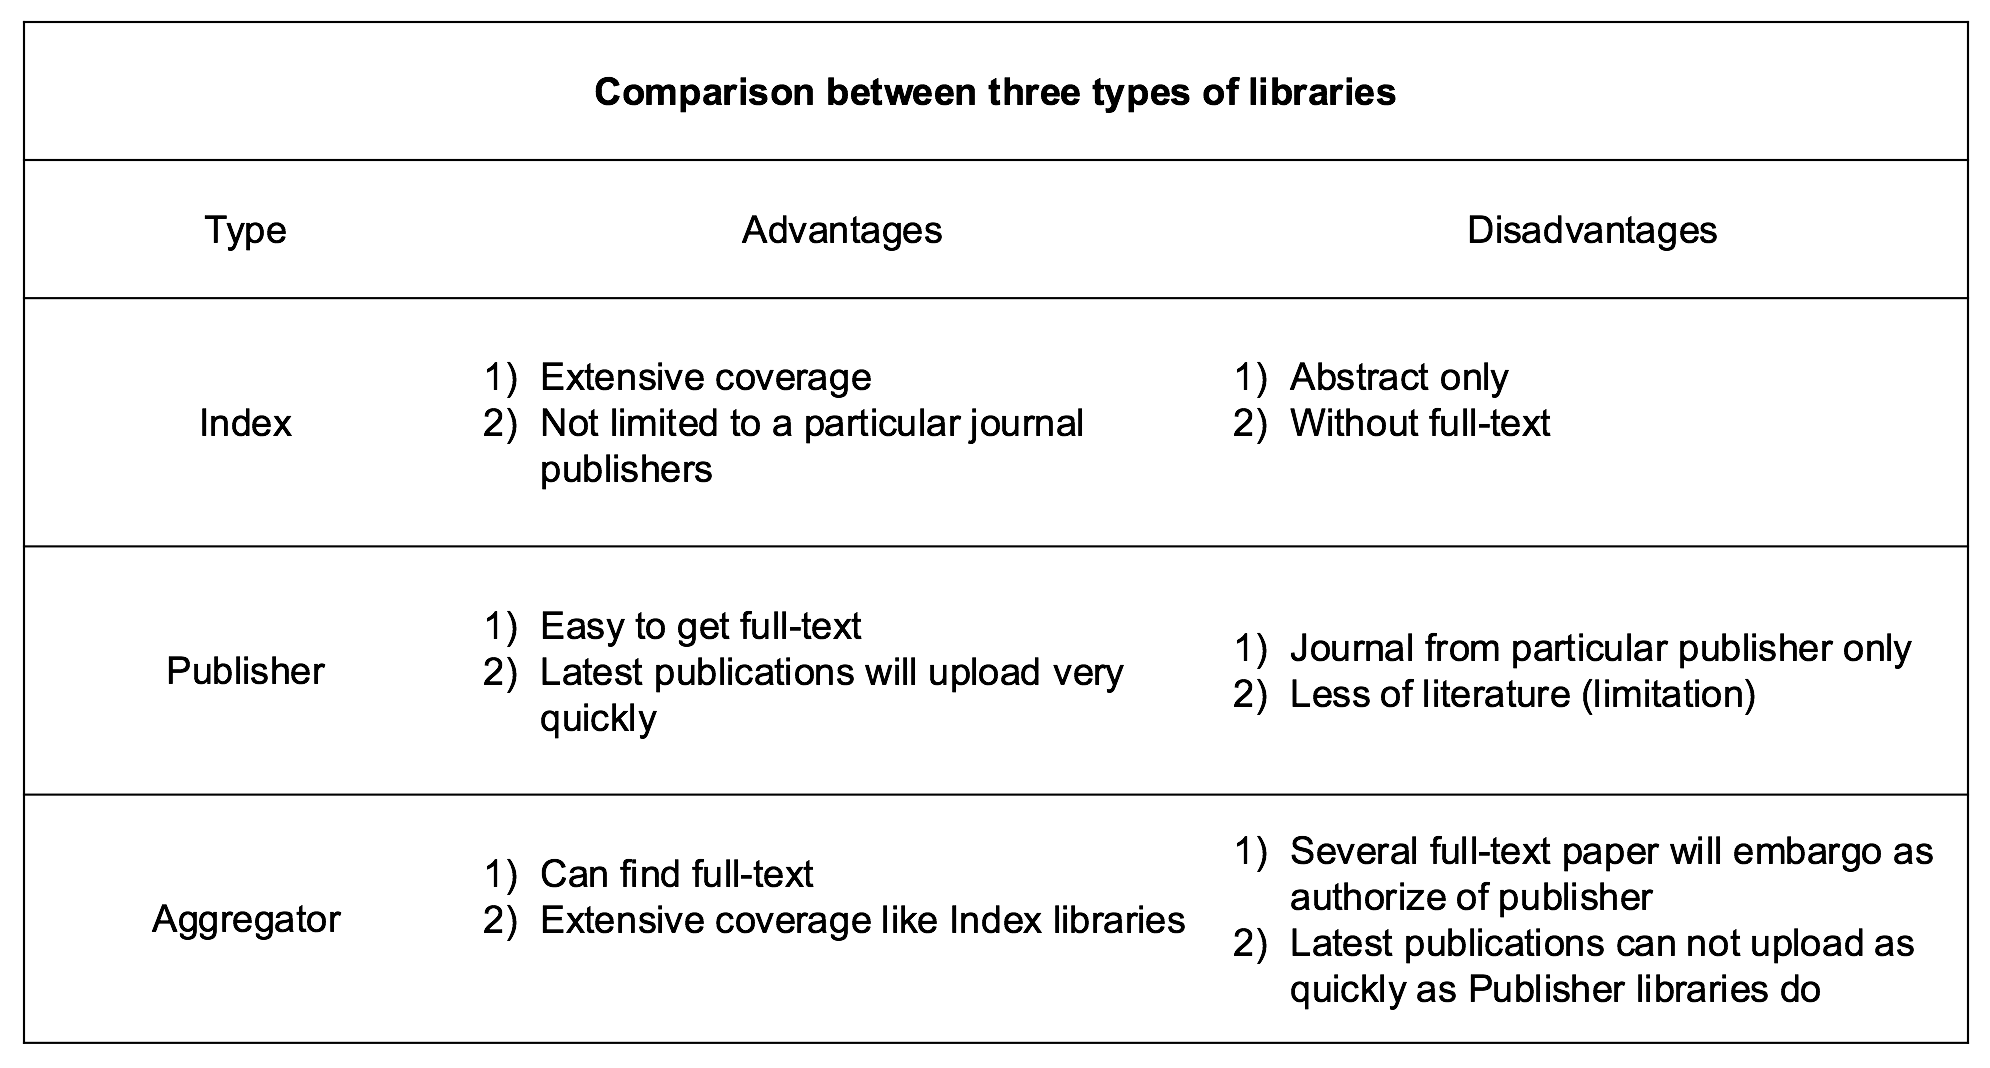
\includegraphics[width=0.8\textwidth]{Wolverine_Background_Chart_1}
	\end{center}
	\caption{Comparison between three types of libraries.\label{WBC1}}
\end{figure*}
\newpage

\subsubsection{Introduction to libraries }

\begin{enumerate}
	
	\item\textbf{PubMed}
	\setlength{\parindent}{1em}
	
	 PMC (PubMed Central) was launched in 2000.
	 PubMed citations often include links to the full-text article on the publishers' web sites or in PMC and the Bookshelf.
	 PubMed is a free library which is used for searching reference papers and abstracts related to the biomedical topics.
	 
	 The largest subset of PubMed is MEDLINE, which is a bibliographic database containing life sciences and biomedical information.
	 Both of them are built by National Library of Medicine. You may limit your search to MEDLINE only in PubMed.
	 A strong feature of PubMed is its ability to link MeSH(Medical Subject Headings) terms automatically. 
	 It is useful for people who want to find the medical articles.
	  
     Simple searches on PubMed can be carried out by entering the key words of a subject into PubMed's search window.
     PubMed translates this initial search formulation and automatically adds field names.
	 Like several libraries, people can find the specific result they desire by adding relevant MeSH terms, synonyms and Boolean operators.	 
	 The design philosophy of PubMed is based on full-text XML files, which are readable by machines, humans and moreover technology independent.
	 
	 PubMed is classified into Index libraries, which is the prime reason that it is not able to provide full text for some papers.
	 The type of database used by PubMed is Microsoft SQL server, which is a relational database to store all of the archives such as XML, images, and PDF files supplementary.
	
	\item\textbf{IEEE Xplore}
	\setlength{\parindent}{1em}	
	
	IEEE is an acronym for Institute of Electrical and Electronics Engineers, which is one of the leading standard organizations in the world. 
	Besides, it is one of the world's largest technical professional organization dedicated to advancing technology for the benefit of humanity. 
	There are more than 420,000 IEEE members in over 160 countries.
	And IEEE Xplore is a scholarly research library formerly known as IEEE/IET Electronic Library (IEL).
	
	The articles covered by IEEE Xplore are mainly from the IEEE and the Institution of Engineering and Technology(IET).
	More than 3.5-million full-text documents are in the field of electrical, engineering, computer science, and electronics are provided in this library. 
	There are many features in IEEE. It can rank the articles according to their click through rates or download times. 
    If some articles are updated by an author, those who set research alert on it will receive a notification through email by IEEE.
    However, some of the features are available for members only.
    Many enterprises and schools are the members of IEEE.
    
	
	\item\textbf{EBSCOhost}
	\setlength{\parindent}{1em}

	EBSCOhost is a popular reference which authorizes users to gain a great many full-text articles from proprietary databases.
	EBSCO Information Services, headquartered in Ipswich, Massachusetts, which is a division of EBSCO Industries Inc., the third largest private company in Birmingham, Alabama with annual sales of nearly $2$ billion according to the BBJ's 2013 Book of Lists.
    EBSCO offers library resources to customers in academic, medical, K–12, public library, law, corporate, and government markets. 
	Its products include EBSCONET, a complete e-resource management system, and EBSCOhost, which supplies a fee-based online research service with 375 full-text databases, a collectionof 600,000-plus ebooks, subject indexes, point-of-care medical references, and an array of historical digital archives.

    In 2010, EBSCO introduced its EBSCO Discovery Service (EDS) to institutions, which allows people to search a portfolio of journals and magazines

	\item\textbf{Google Scholar}
	\setlength{\parindent}{1em}
	
	Google Scholar is a freely accessible web search engine that indexes the full text or metadata of scholarly literature across an array of publishing formats and disciplines. Released in beta in November 2004, the Google Scholar index includes most peer-reviewed online academic journals and books, conference papers, theses and dissertations, preprints, abstracts, technical reports, and other scholarly literature, including court opinions and patents. While Google does not publish the size of Google Scholar's database, third-party researchers estimated it to contain roughly 160 million documents as of May 2014 and an earlier statistical estimate published in PLOS ONE using a Mark and recapture method estimated approximately $80-90$ coverage of all articles published in English with an estimate of 100 million. This estimate also determined how many documents were freely available on the web.
	
	Google Scholar is similar in function to the freely available CiteSeerX and getCITED. It also resembles the subscription-based tools, Elsevier's Scopus and Thomson Reuters' Web of Science.
		
	For further references see \href{https://en.wikipedia.org/wiki/Google_Scholar}{Google-Scholar Wiki}
	
	\item\textbf{Comparison Xplore}\\
	\setlength{\parindent}{1em}
	For comparing please see Matthew2008\cite{Matthew2008}
	

    

\end{enumerate}

